% Indicate the main file. Must go at the beginning of the file.
% !TEX root = ../main.tex

%----------------------------------------------------------------------------------------
% CHAPTER 5
%----------------------------------------------------------------------------------------
\chapter{Results and Discussion} % Main chapter title
\label{Chapter5} % For referencing the chapter elsewhere, use \ref{Chapter5}
All results shown in this section come from data analysis in Appendix \ref{AppendixB}.

\section{Initial Dataset Screening}
\subsubsection*{DEM Screening}
The Initial dataset screen was done in order to evaluate the best DEM and normalization strategy. \footnote{In the legend, you will see a label "residual \_ model \_ mae". This is a typo and should be called Recurrent mae}. The plots and figures, unless otherwise specified, are evaluated using classic MAE (see Eq. \ref{eq:2.3}). 

\begin{figure}[htbp]
	\centering
	\includegraphics[width=0.9\linewidth, height=0.7\linewidth]{"Figures/Results/Initial screening/DEM screening plots/Box_Plot"}
	\caption[Loss over all DEMs]{Loss across all models evaluated over the initial screening datasets}
	\label{fig:dem-screening}
\end{figure}

\begin{figure}[htbp]
	\centering
	\includegraphics[width=0.9\linewidth, height=0.7\linewidth]{"Figures/Results/Initial screening/DEM screening plots/Data_Set_Dem_Screening_Log"}
	\caption[Mean Loss Across DEMs]{Mean loss across all models evaluated over all normalization strategies}
	\label{fig:mean-dem-screening}
\end{figure}

Fig. \ref{fig:dem-screening} shows a box plot for all DEMS. It includes all the normalization strategies (see \ref{methods:inital-screening}). The model used is the DepthwiseCNN model (see \ref{DepthwiseCNN:init}) Fig. \ref{fig:mean-dem-screening} is a bar plot that shows the mean across all DEMs, normalization strategies, and loss functions (see loss functions defined \ref{training:loss}). This was the first test performed. It was done in order to determine which dataset to move forward with. Due to computational limitations and time required for training. Fig. \ref{fig:dem-screening} shows some interesting variation across the datasets. DEM 292 and 709 seemed to show the most promise, but the final decision was to move forward with DEM 292. When we look at the mean values (see Fig. \ref{fig:mean-dem-screening}), We see that DEM 292 has a slightly lower loss than DEM 709. This decision was relatively arbitrary, however, it did have the lowest loss model and showed the fewest outliers. Also the recurrent time step predictions across the board were also the lowest.

\subsubsection*{Normalization strategy}
Fig. \ref{fig:norm-strat-292} shows the loss for each normalization strategy across loss functions. This was used to determine which normalization performed the best overall.

\begin{figure}[tbph]
	\centering
	\includegraphics[width=0.9\linewidth, height=0.5\textheight]{"Figures/Results/Initial screening/Normalization plots/Box_Loss_Norm_strat"}
	\caption[Box plot for different normalization strategies]{Box plot showing the loss for different normalization strategies for DEM 292}
	\label{fig:norm-strat-292}
\end{figure}
The decision for which normalization strategy to use was a challenging task. Due to the nature of the data, where DEM values are extremely large, rainfall values and water depths have a huge range and no real limit. Fig. \ref{fig:norm-strat-292} shows the losses for different normalization strategies. The raw, un normalized data, interestingly, showed a very low loss for the initial model but the recurrent prediction was quite poor and the benchmark models performed the worst overall. The "all Normed" dataset where all features are normalized according to the DEM map showed the greatest variation and seems to be ultimately unpredictable. This leaves us with the independently normalized dataset which shows the least variation and lowest losses. Moving forward, the Independently Normalized dataset is used.
\subsubsection*{Loss Functions}
Table \ref{tab:loss-functions-dem} Hows the loss of all loss functions used for testing over DEM 292. The Column Names are Heuristic (H), Benchmark 1 (BM1), Benchmark 2 (BM2), The current model in question (In this case the initial screening model), and the model but using recurrent prediction.

\begin{table}[h]
	\centering
	\caption{Final Results For Loss Functions Across DEM 292}
	\label{tab:loss-functions-dem}
	\begin{tabular}{p{3cm}ccccc}
		\toprule
		Name &  H &  BM1 &  BM2 &  Model &  Recurrent \\
		\midrule
		MSE &       0.000787 &        0.000914 &        0.002026 &   0.002225 &            0.028407 \\
		MAE &       0.000787 &        0.001607 &        0.003056 &   0.000893 &            0.004070 \\
		MSE AUTO &       0.000787 &        0.001145 &        0.019667 &   0.001983 &           34.082030 \\
		MAE AUTO &       0.000787 &        0.001093 &        0.001836 &   0.000866 &            0.003725 \\
		MSE MAN &       0.000787 &        0.001633 &        0.001352 &   0.000740 &            0.002307 \\
		MAE MAN &       0.000787 &        0.000994 &        0.008186 &   0.000665 &            0.001413 \\
		\bottomrule
	\end{tabular}
\end{table}
Where AUTO and MAN refer to the different regularization done on MSE and MAE. H is the Heuristic, BM1 and BM2 are the benchmark models, Model is the model used during initial screening, Recurrent refers to the recurrent predictions on the test dataset. Fig \ref{fig:loss-comparison-initial} shows this result visually in bar plot. These results determine which loss function to use for the rest of the evaluation.

\begin{figure}[tbph]
	\centering
	\includegraphics[width=0.9\linewidth, height=0.5\textheight]{"Figures/Results/Initial screening/LOSS PLOTS/Loss comparison"}
	\caption[Loss function performance on the individually normed 292 DEM dataset]{The loss for each defined loss function over the individually normalized 292 DEM dataset}
	\label{fig:loss-comparison-initial}
\end{figure}

Choosing the right loss function is a critical task for DL. The problems with classical MAE and MSE, which are essentially the only options for regression tasks like this (when dealing with two-dimensional, multi-channel tensors), in this case is their bias towards predicting 0 water depth. The nature of datasets like this, is its un balanced nature. Looking at the rainfall events (see Fig. \ref{fig:4.2} and \ref{fig:4.4}), we see there are many moments where there is very small or no rainfall. On top of that, the simulated data thresholds water depth. When water depth is less than 0.01 m, it outputs 0 (see Eq. \ref{eq:thresholdwd}).

\begin{equation}
	\label{eq:thresholdwd}
	Wd_{new} = \begin{cases}
		0, & \text{if } Wd < 0.01 \\
		Wd, & \text{Otherwise}
	\end{cases}
\end{equation}

Table \ref{tab:loss-functions-dem} shows the loss's across models for each loss function variation across the independently normalized dataset for DEM 292 (see Fig \ref{fig:loss-comparison-initial}) We see that MSE loss doesn't generally perform as well as MAE. This might be because the metric chosen was mae, so there is potential for bias. Weights chosen for the  manual weighted loss functions were 0.8 zero weight and 0.2 non zero weight. This may seem counter intuitive to what is mentioned above but it still performed the best. This is because predicting 0 change in water depth outperformed the Heuristic. MSE and MSE AUTO variations performed the worst by a large margin. While manual MAE performed the best. Therefore, we move forward with this variation.

\section{Model Complexity and Hyperparameter tuning}

\subsubsection*{Predicting Water Depth}
Two methods were evaluated. Models predicting water depth directly and models predicting the difference in water depth. Fig \ref{fig:diffvsnodiff} shows a box plot of loss for predicting water depth versus predicting the difference in water depth between time steps. It is done across different learning rates, model complexities and epoch number (2 and 10 epochs).
\begin{figure}[tbph]
	\centering
	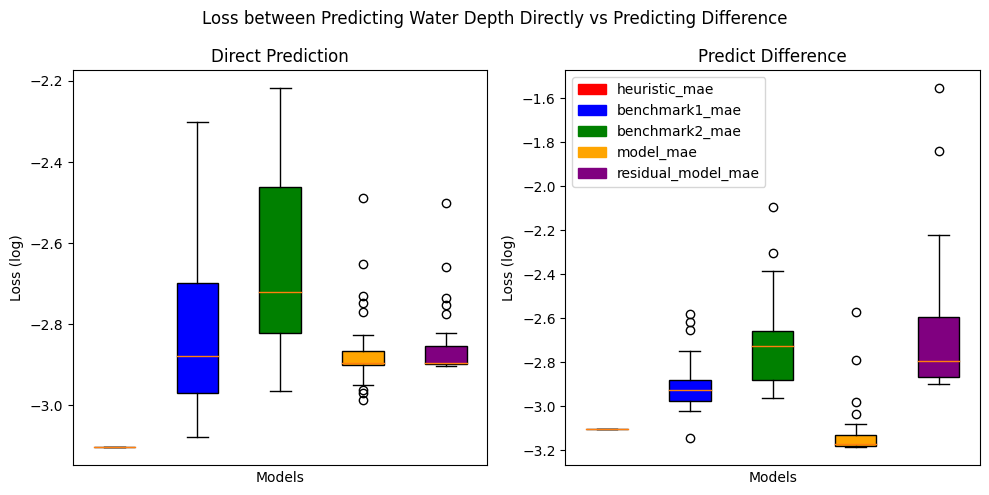
\includegraphics[width=0.8\linewidth, height=0.3\textheight]{Figures/Results/Diff_Complexity_Lr_Epochs/Predicting_Diff/box_dif_v_no_diff}
	\caption[Predicting water depth difference vs predicting water depth directly]{Loss for predicting water depth directly vs predicting the difference in water depth}
	\label{fig:diffvsnodiff}
\end{figure}

Fig \ref{fig:diffvsnodiff} shows that models trained to predict water depth directly have much more variability. Loss  for predicting a single time step has more outliers and performs worse on average than predicting the difference in water depth. However, it seems that recurrent time step prediction performs better. Only models that predict difference in water depth over a single time step perform better than the heuristic. Based on these results, further evaluation is only based on predicting difference in water depth.

\subsubsection*{Model Complexity, Predicting Difference in Water Depth}
Fig. \ref{fig:depthwise-complexity} shows the loss of different model complexities across epochs and learning rates. The shallow DepthwiseCNN model seems to show the best results. All model complexities out-perform the heuristic. Unfortunately, whilst generating data and deciding which models to do further testing on, only the best models were considered. In this case, the best performing model was a medium complexity model (see 5th row of Table \ref{tab:best_ss}). So further work was done on the medium complexity model. Further testing should be done on a simpler model, especially where the recurrent (and most useful) loss is concerned. 
\begin{figure}[tbph]
	\centering
	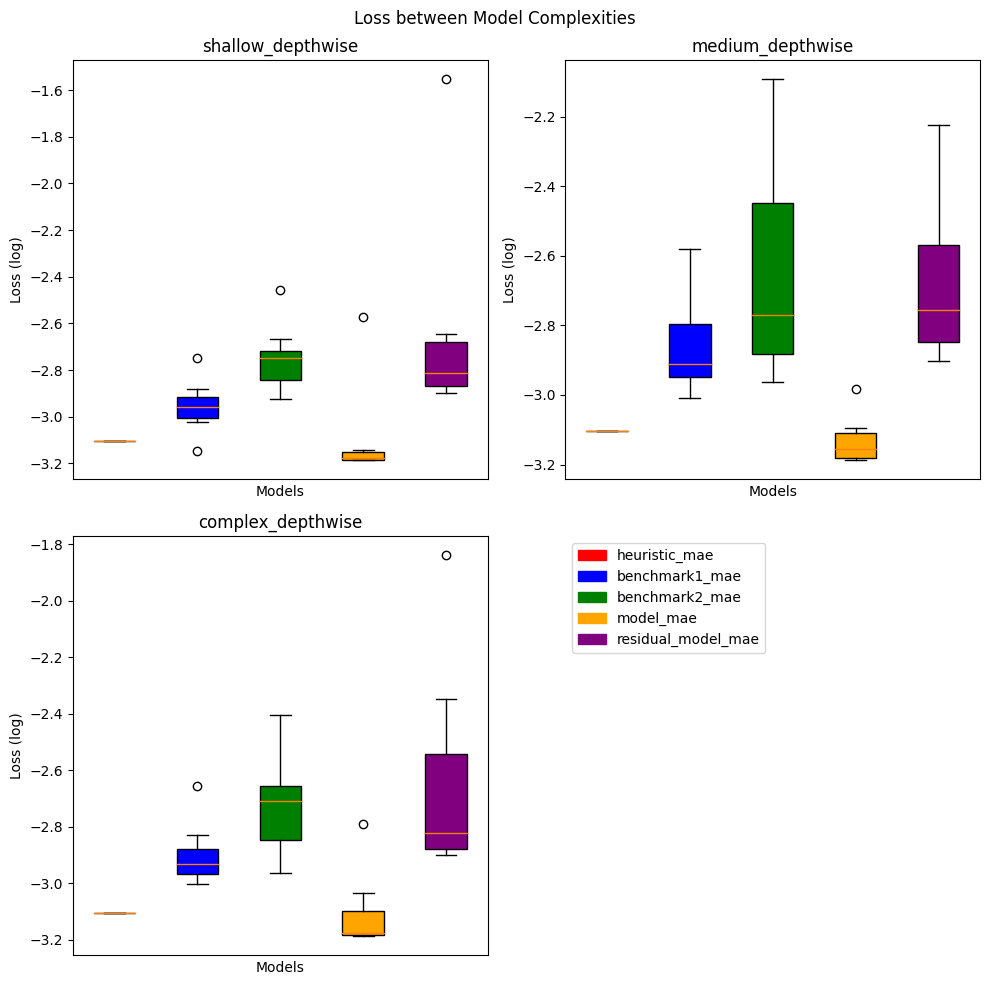
\includegraphics[width=0.7\linewidth, height=0.4\textheight]{Figures/Results/Diff_Complexity_Lr_Epochs/Complexity/Box_model_complexity}
	\caption[Loss Depending on Model Complexity for DepthwiseCNN]{Loss for different model complexities that predict water difference}
	\label{fig:depthwise-complexity}
\end{figure}


\subsubsection*{Epochs and Learning Rate for Medium Complexity DepthwiseCNN}
Fig \ref{fig:epochs} shows the model loss for the medium complexity DepthwiseCNN. This is across a variety of learning rates, which are shown in Table \ref{tab:lr}. There was very little difference between the epochs. A reason for this might be due to the stop loss callback option used during training. Overall, across all testing, models struggled to learn anything. A reason for this may be due to being trapped in a local minima from the start. If the model was predicting no change, the loss was very low and even outperformed the heuristic. Fig \ref{fig:egloss-epochs} shows an example loss across all models (benchmark and DepthwiseCNN model).

\begin{figure}[tbph]
	\centering
	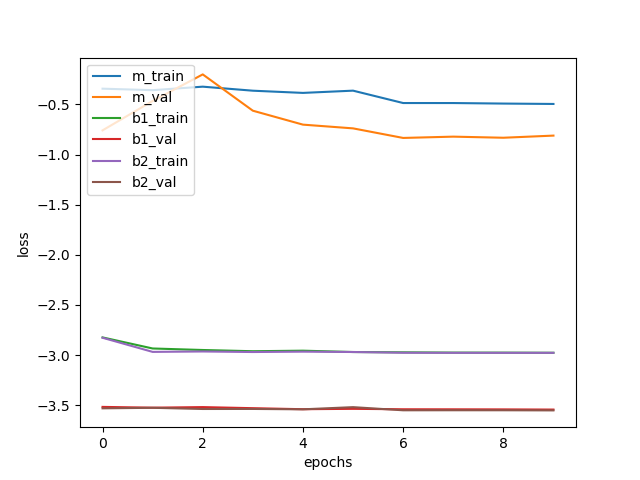
\includegraphics[width=0.6\linewidth, height=0.6\textheight]{Figures/Results/Diff_Complexity_Lr_Epochs/Epochs_Lr/medium_depthwise_diff_train_2_custom_mae_weighted_2e-3_more_epochs_norm_independant_292_training}
	\caption[Example Loss for Medium depthwise model and benchmarks]{Example training loss for medium depthwise model and benchmarks}
	\label{fig:egloss-epochs}
\end{figure}


\begin{figure}[tbph]
	\centering
	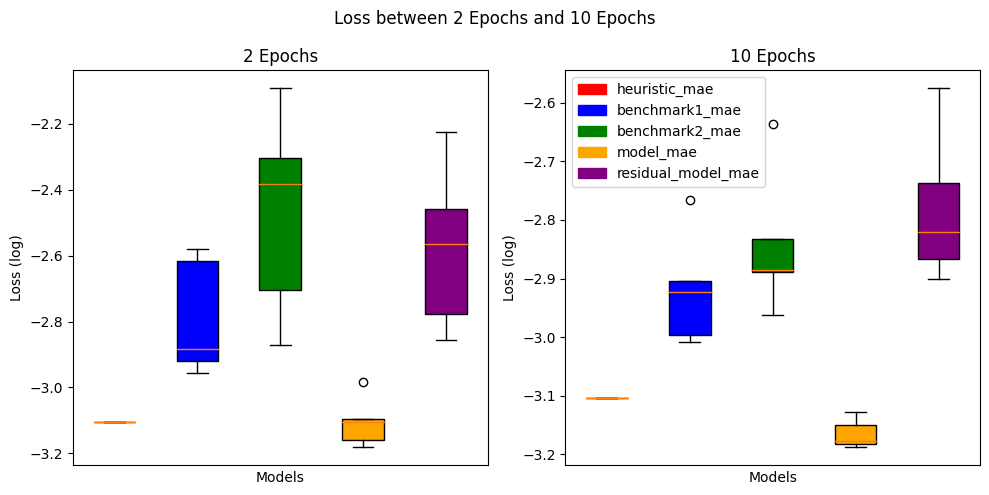
\includegraphics[width=0.8\linewidth, height=0.3\textheight]{Figures/Results/Diff_Complexity_Lr_Epochs/Epochs_Lr/Box_epochs}
	\caption[Loss between two different Epochs]{Loss for medium complexity DepthwiseCNN model over two different epochs}
	\label{fig:epochs}
\end{figure}

\begin{table}[htbp]
	\centering
	\caption{Final losses for different learning rate with Medium Complexity}
	\label{tab:lr}
	\begin{tabular}{p{2cm}ccccc}
		\toprule
		Name &  H &  BM1 &  BM2 &  Model &  Recurrent \\
		\midrule
		1e-3 &       0.000787 &        0.001194 &        0.001092 &   0.000665 &            0.001510 \\
		2e-3 &       0.000787 &        0.001010 &        0.001302 &   0.000658 &            0.001360 \\
		1e-4 &       0.000787 &        0.001714 &        0.002307 &   0.000648 &            0.001254 \\
		1e-2 &       0.000787 &        0.001246 &        0.001473 &   0.000744 &            0.002659 \\
		5e-4 &       0.000787 &        0.000982 &        0.001290 &   0.000707 &            0.001836 \\
		\bottomrule
	\end{tabular}
\end{table}

\subsubsection*{Optimal Weights for MAE}
Table \ref{tab:weights} shows the loss for different weights for the manual MAE loss function. (see Fig. \ref{fig:MAE-weights-init} for a visual representation). 
\begin{figure}[tbph]
	\centering
	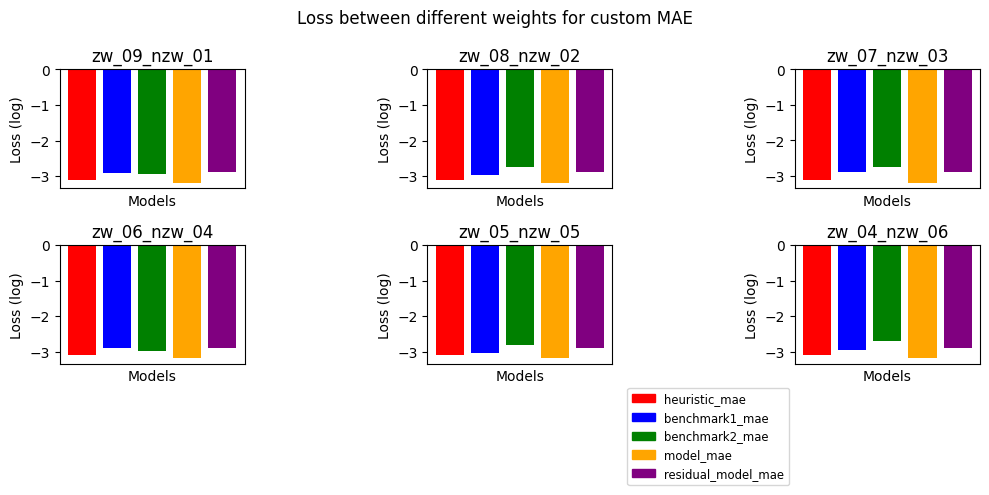
\includegraphics[width=0.9\linewidth, height=0.5\textheight]{Figures/Results/Shuffle_Weights/weights/weights}
	\caption[Loss for Different Weights of MAE]{Loss for Different Weights of MAE}
	\label{fig:MAE-weights-init}
\end{figure}

\begin{table}[htbp]
	\centering
	\caption{The loss for different weightings in the MAE manuel loss function}
	\label{tab:weights}
	\begin{tabular}{p{2cm}ccccc}
		\toprule
		Name &  H &  BM1 &  BM2 &  Model &  Recurrent \\
		\midrule
		09|01 &       0.000787 &        0.001204 &        0.001137 &   0.000655 &            0.001322 \\
		08|02 &       0.000787 &        0.001042 &        0.001830 &   0.000654 &            0.001335 \\
		07|03 &       0.000787 &        0.001276 &        0.001845 &   0.000649 &            0.001267 \\
		06|04 &       0.000787 &        0.001248 &        0.001051 &   0.000652 &            0.001302 \\
		05|05 &       0.000787 &        0.000894 &        0.001517 &   0.000649 &            0.001260 \\
		04|06 &       0.000787 &        0.001127 &        0.002029 &   0.000649 &            0.001263 \\
		\bottomrule
	\end{tabular}
\end{table}
Where the name indicates zero weight and non zero weight respectively. (eg. zero weight of 0.9 and non zero weight of 0.1, i.e. 0.9|0.1)
\subsubsection*{Shuffling the Data}]
Table \ref{tab:suffle} shows the results of shuffling the data using the function 'train \_ test \_ split()' from the python library sklearn with kwarg** shuffle=True.
\begin{table}[h]
	\centering
	\caption{The loss for shuffled or not shuffled}
	\label{tab:suffle}
	\begin{tabular}{p{2cm}ccccc}
		\toprule
		Name &  H &  BM1 &  BM2 &  Model &  Recurrent \\
		\midrule
		Shuffled &       0.000787 &        0.002165 &        0.001247 &   0.000648 &            0.001255 \\
		Sequential &       0.000787 &        0.001578 &        0.001307 &   0.000649 &            0.001263 \\
		\bottomrule
	\end{tabular}
\end{table}

\section{Additional Features}

\begin{figure}[tbph]
	\centering
	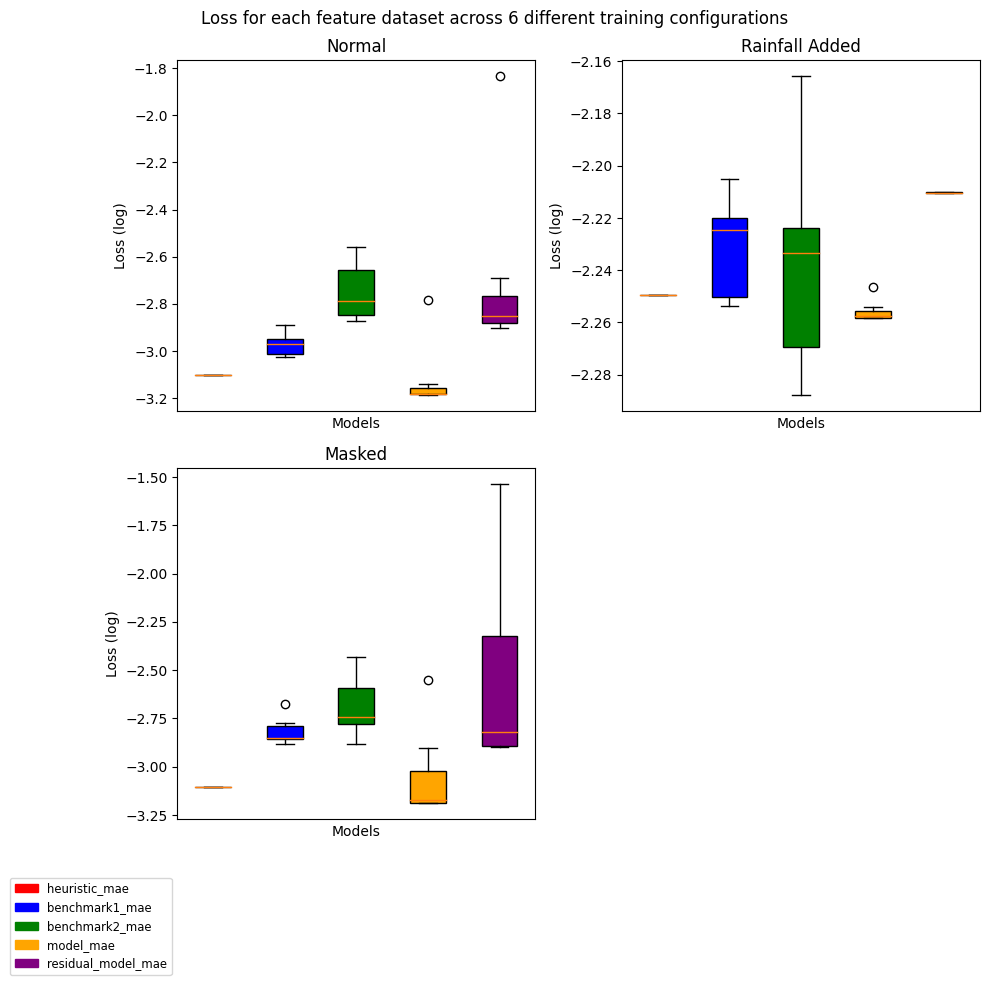
\includegraphics[width=0.7\linewidth, height=0.5\textheight]{Figures/Results/feature_manip/feature_manip_across_lr}
	\caption[Loss For Three different Datasets With Different Features]{Loss for Three different Datasets with Different Features across different training configurations}
	\label{fig:norm-rain-mask-init}
\end{figure}


\begin{table}[htbp]
	\centering
	\caption{Six training configurations testing two different weights for MAE Manuel and three lr across the original, normalized dataset}
	\label{tab:weighte_lr}
	\begin{tabular}{p{2cm}ccccc}
		\toprule
		Name &  H &  BM1 &  BM2 &  Model &  Recurrent \\
		\midrule
		w11 &       0.000787 &        0.001163 &        0.001336 &   0.000669 &            0.001453 \\
		w12 &       0.000787 &        0.000958 &        0.001636 &   0.000726 &            0.002032 \\
		w13 &       0.000787 &        0.001284 &        0.001447 &   0.000658 &            0.001350 \\
		w21 &       0.000787 &        0.001067 &        0.002772 &   0.001642 &            0.014677 \\
		w22 &       0.000787 &        0.000942 &        0.002398 &   0.000657 &            0.001403 \\
		w23 &       0.000787 &        0.000990 &        0.002026 &   0.000648 &            0.001255 \\
		\bottomrule
	\end{tabular}
\end{table}

Where the first number indicates the weight ratio,
\begin{enumerate}
	\item 0.5|0.5
	\item  0.2|0.8
\end{enumerate}

And the second number indicates the learning rate,
\begin{enumerate}
	\item  1e-2
	\item  1e-3
	\item  1e-4
\end{enumerate}
For example [w11] from Table \ref{tab:weighte_lr} w11 would be weight ratio of 0.5 zero weight and 0.5 non zero weight, with a learning rate of 1e-2.


\section{Inception Inspired Model}
In this section, column names are w1, w2, w3, They represent the following training regime,
\begin{enumerate}
	\item[w1] 20 Epochs, learning rate of 1e-2, manual MAE with zero weight 0,2 and non zero weight of 0,8
	\item[w2] 20 Epochs, learning rate of 1e-3, manual MAE with zero weight 0,2 and non zero weight of 0,8
	\item[w3] 20 Epochs, learning rate of 1e-3, manual MAE with zero weight 0,1 and non zero weight of 0,9
\end{enumerate}
\subsubsection*{Training Across Different Feature Datasets}
Fig. \ref{fig:incep-normaldset}, \ref{fig:incep-rfdset}, \ref{fig:incep-maskdset} are the plots showing the losses of two different model complexities, simple and medium, across varying learning rates and weights for the manual MAE (see above).
\begin{figure}[tbph]
	\centering
	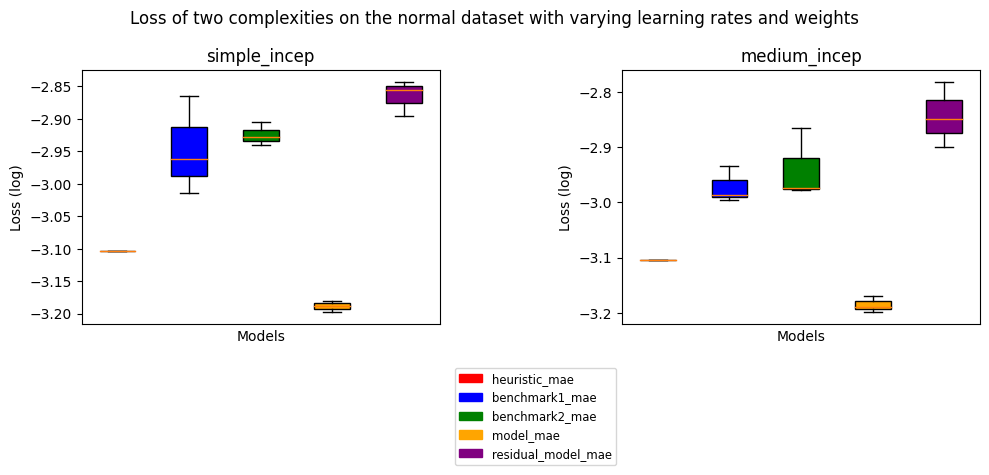
\includegraphics[width=0.8\linewidth, height=0.3\textheight]{Figures/Results/Inception_model/normal_dataset}
	\caption[Loss for Inception Inspired model for two different complexities on the normal dataset]{Loss for Inception Inspired model for two different complexities on the normal dataset}
	\label{fig:incep-normaldset}
\end{figure}


\begin{figure}[tbph]
	\centering
	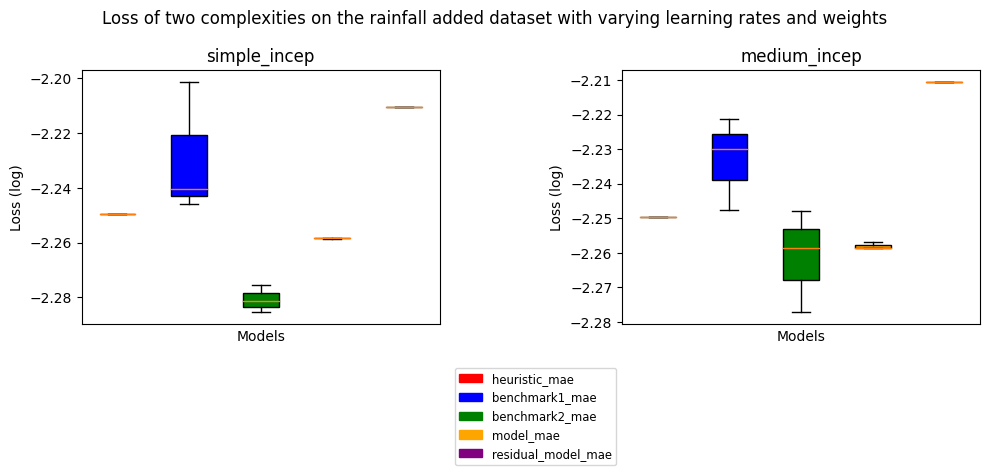
\includegraphics[width=0.8\linewidth, height=0.3\textheight]{Figures/Results/Inception_model/rainfall_dataset}
	\caption[Loss for Inception Inspired model for two different complexities on the added rainfall dataset]{Loss for Inception Inspired model for two different complexities on the added rainfall dataset}
	\label{fig:incep-rfdset}
\end{figure}

\begin{figure}[tbph]
	\centering
	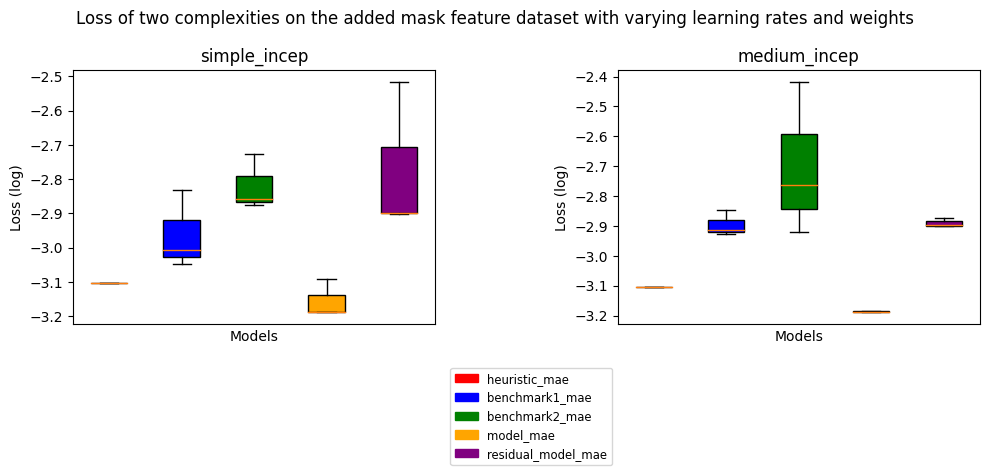
\includegraphics[width=0.8\linewidth, height=0.3\textheight]{Figures/Results/Inception_model/mask_dataset}
	\caption[Loss for Inception Inspired model for two different complexities on the added mask dataset]{Loss for Inception Inspired model for two different complexities on the added masked dataset}
	\label{fig:incep-maskdset}
\end{figure}

\subsubsection*{Simple model}
\begin{table}[htbp]
	\centering
	\caption{Three training configurations on the normal dataset for simple inception based model}
	\label{tab:simple_normal}
	\begin{tabular}{p{2cm}ccccc}
		\toprule
		Name &  H &  BM1 &  BM2 &  Model &  Recurrent \\
		\midrule
		w1 &       0.000787 &        0.000966 &        0.001179 &   0.000661 &            0.001437 \\
		w2 &       0.000787 &        0.001093 &        0.001247 &   0.000648 &            0.001272 \\
		w3 &       0.000787 &        0.001366 &        0.001146 &   0.000634 &            0.001396 \\
		\bottomrule
	\end{tabular}
\end{table}

\begin{table}[htbp]
	\centering
	\caption{Three training configurations on the rainfall added dataset for simple inception based model}
	\label{tab:simple_rf}
	\begin{tabular}{p{2cm}ccccc}
		\toprule
		Name &  H &  BM1 &  BM2 &  Model &  Recurrent \\
		\midrule
		w1 &       0.005629 &        0.005676 &        0.005305 &   0.005517 &            0.006159 \\
		w2 &       0.005629 &        0.006293 &        0.005231 &   0.005514 &            0.006159 \\
		w3 &       0.005629 &        0.005750 &        0.005183 &   0.005519 &            0.006159 \\
		\bottomrule
	\end{tabular}
\end{table}

\begin{table}[htbp]
	\centering
	\caption{Three training configurations on the mask added dataset for simple inception based model}
	\label{tab:simple_mask}
	\begin{tabular}{p{2cm}ccccc}
		\toprule
		Name &  H &  BM1 &  BM2 &  Model &  Recurrent \\
		\midrule
		w1 &       0.000787 &        0.000986 &        0.001333 &   0.000811 &            0.003052 \\
		w2 &       0.000787 &        0.001469 &        0.001390 &   0.000648 &            0.001262 \\
		w3 &       0.000787 &        0.000897 &        0.001878 &   0.000648 &            0.001253 \\
		\bottomrule
	\end{tabular}
\end{table}


\subsubsection*{Medium Model}
The Medium complexity model increases parameter count slightly. The results are shown below
\begin{table}[htbp]
	\centering
	\caption{Three training configurations on the normal dataset for medium inception based model}
	\label{tab:medium_normal}
	\begin{tabular}{p{2cm}ccccc}
		\toprule
		Name &  H &  BM1 &  BM2 &  Model &  Recurrent \\
		\midrule
		w1 &       0.000787 &        0.001032 &        0.001054 &   0.000676 &            0.001655 \\
		w2 &       0.000787 &        0.001166 &        0.001064 &   0.000632 &            0.001418 \\
		w3 &       0.000787 &        0.001011 &        0.001362 &   0.000648 &            0.001258 \\
		\bottomrule
	\end{tabular}
\end{table}

\begin{table}[htbp]
	\centering
	\caption{Three training configurations on the rainfall added dataset for medium inception based model}
	\label{tab:medium_rf}
	\begin{tabular}{p{2cm}ccccc}
		\toprule
		Name &  H &  BM1 &  BM2 &  Model &  Recurrent \\
		\midrule
		w1 &       0.005629 &        0.005655 &        0.005513 &   0.005534 &            0.006159 \\
		w2 &       0.005629 &        0.006006 &        0.005282 &   0.005514 &            0.006160 \\
		w3 &       0.005629 &        0.005888 &        0.005650 &   0.005514 &            0.006160 \\
		\bottomrule
	\end{tabular}
\end{table}

\begin{table}[htbp]
	\centering
	\caption{Three training configurations on the mask added dataset for medium inception based model}
	\label{tab:medium_mask}
	\begin{tabular}{p{2cm}ccccc}
		\toprule
		Name &  H &  BM1 &  BM2 &  Model &  Recurrent \\
		\midrule
		w1 &       0.000787 &        0.001427 &        0.003831 &   0.000654 &            0.001342 \\
		w2 &       0.000787 &        0.001183 &        0.001719 &   0.000647 &            0.001254 \\
		w3 &       0.000787 &        0.001222 &        0.001197 &   0.000650 &            0.001267 \\
		\bottomrule
	\end{tabular}
\end{table}

\section{Final Results Overall}
\begin{table}[htbp]
	\centering
	\caption{The Top Five Models Across all Training SS}
	\label{tab:best_ss}
	\begin{tabular}{p{2cm}ccccc}
		\toprule
		Name &  H &  BM1 &  BM2 &  Model &  Recurrent \\
		\midrule
		1 &       0.000787 &        0.001166 &        0.001064 &   0.000632 &            0.001418 \\
		2 &       0.000787 &        0.001366 &        0.001146 &   0.000634 &            0.001396 \\
		3 &       0.000787 &        0.001183 &        0.001719 &   0.000647 &            0.001254 \\
		4 &       0.000787 &        0.001011 &        0.001362 &   0.000648 &            0.001258 \\
		5 &       0.000787 &        0.002165 &        0.001247 &   0.000648 &            0.001255 \\
		\bottomrule
	\end{tabular}
\end{table}
Table \ref{tab:best_ss} shows the top performing models for predicting a single time step (SS) ahead, overall across all testing. The Name column has the following keys,
\begin{enumerate}
	\item Medium Complexity Inception Inspired Model on the normalized dataset with the original three features. Trained with 20 Epochs, a learning rate of 1e-3, manual MAE loss with zero weighting of 0,2 and non zero weighting 0,8.
	\item Simple Complexity Inception Inspired Model on the normalized dataset. Trained with 20 Epochs, a learning rate of 1e-3, manual MAE loss with zero weighting of 0,1 and non zero weighting 0,9.
	\item Medium Complexity Inception Inspired Model on the normalized dataset with an additional mask feature. Trained with 20 Epochs, a learning rate of 1e-3, manual MAE loss with zero weighting of 0,2 and non zero weighting 0,8.
	\item Medium Complexity Inception Inspired Model on the normalized dataset with the original three features. Trained with 20 Epochs, a learning rate of 1e-3, manual MAE loss with zero weighting of 0,1 and non zero weighting 0,9.
	\item Medium complexity DepthwiseCNN model on the normalized dataset with original features. Trained with 8 Epochs,a learning rate of 1e-4, manual MAE lsos with zero weighting of 0,5 and non zero weighting of 0,5.
\end{enumerate}

\begin{table}[htbp]
	\centering
	\caption{The Top Five Models Across all Training For Recurrent Steps}
	\label{tab:best_r}
	\begin{tabular}{p{2cm}ccccc}
		\toprule
		Name &  H &  BM1 &  BM2 &  Model &  Recurrent \\
		\midrule
		1 &       0.000787 &        0.001502 &        0.001632 &   0.001253 &            0.001253 \\
		2 &       0.000787 &        0.000897 &        0.001878 &   0.000648 &            0.001253 \\
		3 &       0.000787 &        0.001183 &        0.001719 &   0.000647 &            0.001254 \\
		4 &       0.000787 &        0.002816 &        0.003378 &   0.001254 &            0.001254 \\
		5 &       0.000787 &        0.001714 &        0.002307 &   0.000648 &            0.001254 \\
		\bottomrule
	\end{tabular}
\end{table}
Table \ref{tab:best_r} shows the top five models based on recurrent water depth prediction across all training. The name column has the following key-value pairs,
\begin{enumerate}
	\item Medium Complexity DepthwiseCNN model predicting water depth directly. Trained on the normalized dataset with 10 epochs, a learning rate of 1e-4. 
	\item Simple Complexity Inception Inspired model the normalized dataset with the added mask feature. Trained with 20 Epochs, a learning rate of 1e-3, manual MAE loss with zero weighting of 0,1 and non zero weighting 0,9.
	\item Medium Complexity Inception Inspired Model on the normalized dataset with the  added mask feature, predicting difference in water depth. Trained with 20 Epochs, a learning rate of 1e-3, manual MAE loss with zero weighting of 0,2 and non zero weighting 0,8.
	\item Medium Complexity DepthwiseCNN model predicting water depth directly. Trained on the normalized dataset with 2 epochs, a learning rate of 1e-4.
	\item Medium Complexity DepthwiseCNN model predicting the difference in  water depth. Trained on the normalized dataset with 10 epochs, a learning rate of 1e-4.
\end{enumerate}

\begin{table}[htbp]
	\centering
	\caption{The Worst Five Models Across all Training For SS}
	\label{tab:worstss}
	\begin{tabular}{p{2cm}ccccc}
		\toprule
		Name &  H &  BM1 &  BM2 &  Model &  Recurrent \\
		\midrule
		1 &       0.002279 &       81.628900 &      106.629910 &  44.619150 &          648.459210 \\
		2 &       0.002279 &       78.769480 &      111.990715 &  32.265385 &          379.157455 \\
		3 &       0.002551 &       14.399827 &       25.591928 &  16.135822 &          187.824300 \\
		4 &       0.002551 &       21.657652 &       24.267190 &   8.066945 &          101.351124 \\
		5 &       0.002551 &       18.857510 &       27.992000 &   5.856058 &           83.558502 \\
		\bottomrule
	\end{tabular}

\end{table}
Table \ref{tab:worstss} shows the worst five performing models for predicting a single time step (SS) ahead, overall across all testing. The Name column has the following keys,
\begin{enumerate}
	\item Inital Depthwise Model using classic MSE on the DEM 26 dataset where everything was min max normalized using the DEM. Trained using 2 Epochs, default learning rate of 1e-3.
	\item Inital Depthwise Model using manual MSE on the DEM 26 dataset where everything was min max normalized using the DEM. Trained using 2 Epochs, default learning rate of 1e-3. zero weight of 0.8 and non zero weight of 0.2.
	\item Inital Depthwise Model using classic MSE on the DEM 819 dataset where everything was min max normalized using the DEM. Trained using 2 Epochs, default learning rate of 1e-3.
	\item Inital Depthwise Model using  manual MSE on the DEM 819 dataset where everything was min max normalized using the DEM. Trained using 2 Epochs, default learning rate of 1e-3. zero weight of 0.8 and non zero weight of 0.2.
	\item Inital Depthwise Model using  auto MSE on the DEM 819 dataset where everything was min max normalized using the DEM. Trained using 2 Epochs, default learning rate of 1e-3.
\end{enumerate}


\begin{table}[htbp]
	\centering
	\caption{The Worst Five Models Across all Training For Recurrent Steps}
	\label{tab:worstr}
	\begin{tabular}{p{2cm}ccccc}
		\toprule
		Name &  H &  BM1 &  BM2 &  Model &  Recurrent \\
		\midrule
		1 &       0.002279 &       81.628900 &      106.629910 &  44.619150 &          648.459210 \\
		2 &       0.002279 &       78.769480 &      111.990715 &  32.265385 &          379.157455 \\
		3 &       0.002551 &       14.399827 &       25.591928 &  16.135822 &          187.824300 \\
		4 &       0.002440 &        4.586013 &       38.804940 &   4.971159 &          164.466783 \\
		5 &       0.001346 &        0.001753 &        0.002407 &   0.002654 &          119.582068 \\
		\bottomrule
	\end{tabular}
\end{table}

Table \ref{tab:worstr} shows the worst five performing models for predicting recurrent time steps ahead, overall across all testing. The Name column has the following keys,
\begin{enumerate}
	\item Inital Depthwise Model using classic MSE on the DEM 26 dataset where everything was min max normalized using the DEM. Trained using 2 Epochs, default learning rate of 1e-3.
	\item Inital Depthwise Model using manual MSE on the DEM 26 dataset where everything was min max normalized using the DEM. Trained using 2 Epochs, default learning rate of 1e-3. zero weight of 0.8 and non zero weight of 0.2.
	\item Inital Depthwise Model using classic MSE on the DEM 819 dataset where everything was min max normalized using the DEM. Trained using 2 Epochs, default learning rate of 1e-3.
	\item Inital Depthwise Model using  auto MAE on the DEM 292 dataset where everything was min max normalized using the DEM. Trained using 2 Epochs, default learning rate of 1e-3.
	\item Inital Depthwise Model using  auto MSE on the DEM 819 dataset where features are normalized independently. Trained using 2 Epochs, default learning rate of 1e-3.
\end{enumerate}

The following plots where created after all initial testing to try and reproduce the models. Fig. \ref{fig:BRMR} Shows the water depths the true values, heuristic model, and deep learning model of a random cell in the test set using a recurrent time step method prediction. The model used was the best performing model for a single time step prediction.  (see Table. \ref{tab:best_r}). Fig. \ref{fig:BRMS} Shows the same plot but prediciting a single time step ahead. Fig. \ref{fig:BSMR} and \ref{fig:BSMS} Are the plots respectively but using the best single time step model (see Table. \ref{tab:best_ss}).

\begin{figure}[tbph]
	\centering
	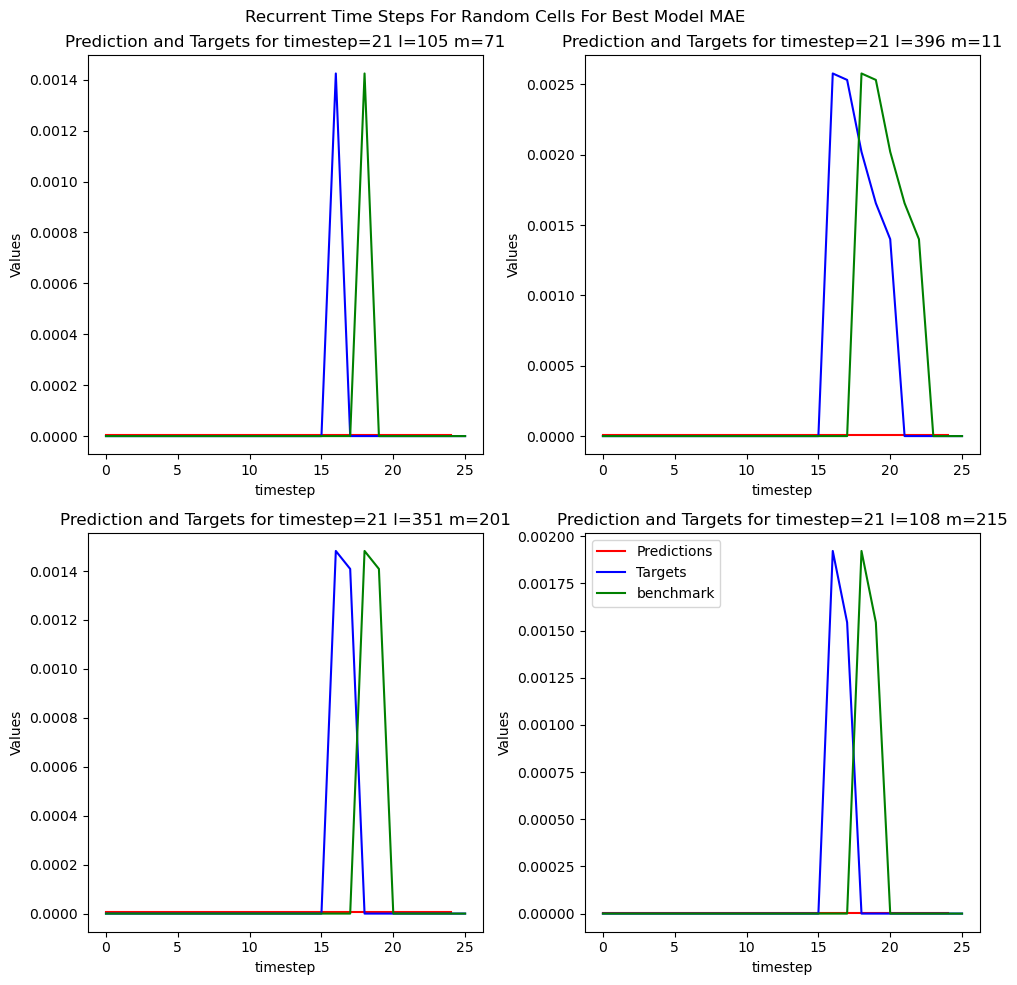
\includegraphics[width=0.8\linewidth, height=0.3\textheight]{Figures/Results/Final_Results/Best_Model_recurrentMAE_recurrent_random_cell}
	\caption[Best Recurrent MAE random cell over time]{Water Depth Predictions recurrently over the test set timesteps}
	\label{fig:BRMR}
\end{figure}



\begin{figure}[tbph]
	\centering
	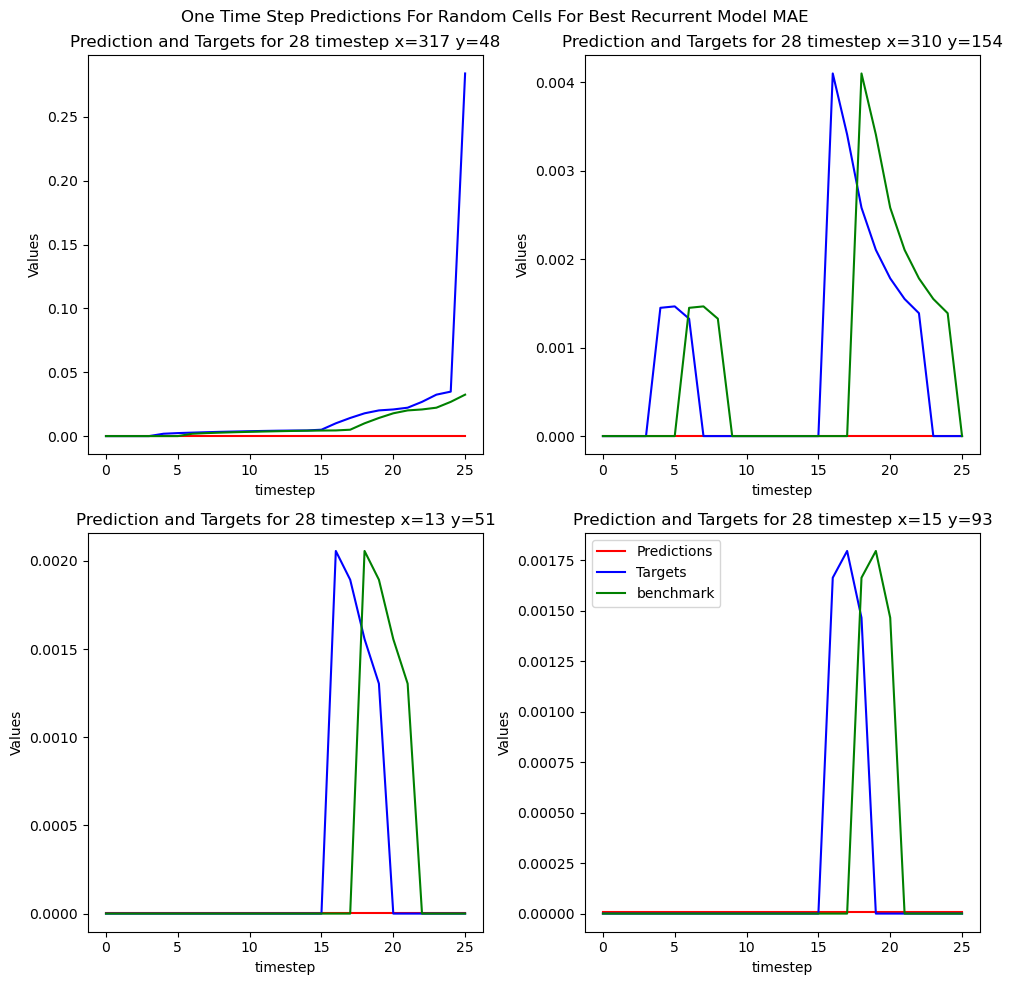
\includegraphics[width=0.8\linewidth, height=0.3\textheight]{Figures/Results/Final_Results/Best_Model_recurrentMAE_SS_random_cell}
	\caption[Best Recurrent Loss on single time step predictions over test set]{Best Recurrent Loss on single time step predictions over test set}
	\label{fig:BRMS}
\end{figure}


\begin{figure}[tbph]
	\centering
	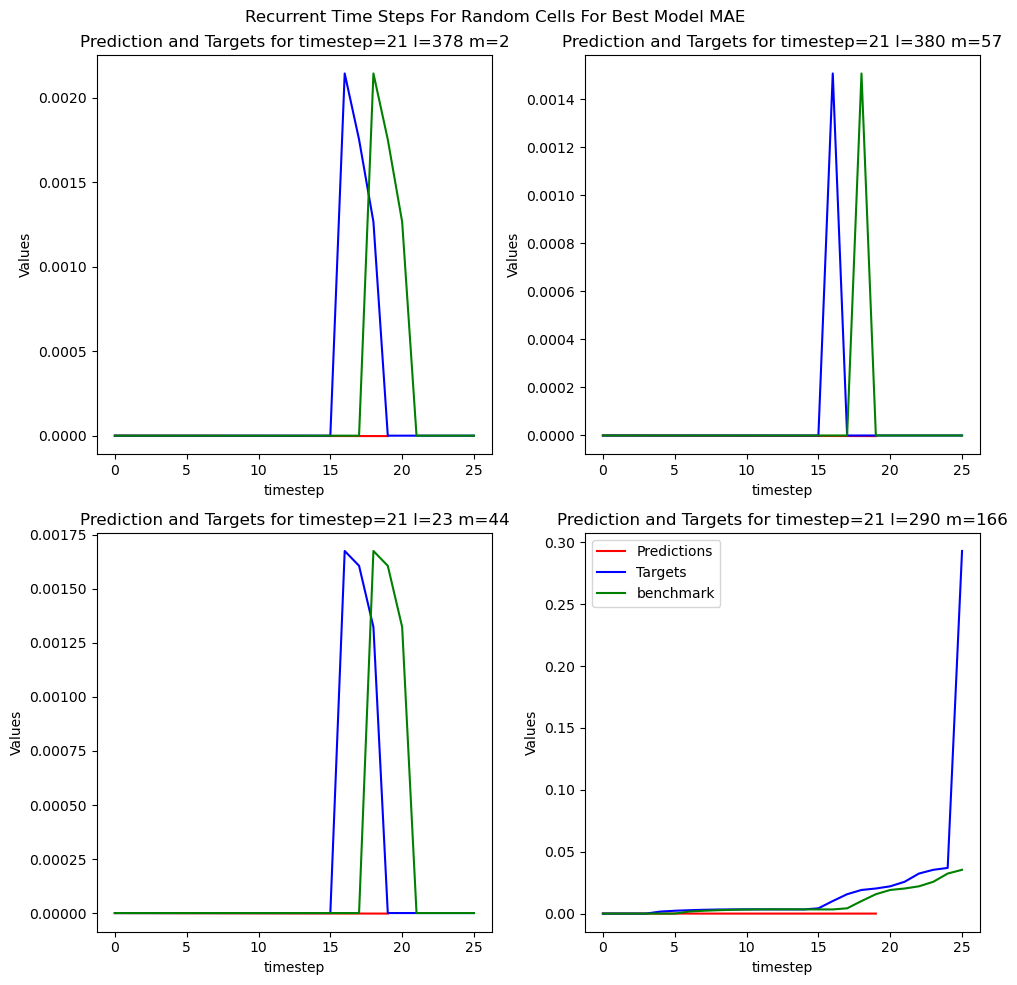
\includegraphics[width=0.8\linewidth, height=0.3\textheight]{Figures/Results/Final_Results/Best_Model_SS_recurrent_random_cell}
	\caption[Best single step model on test set predicting water depth for recurrent time steps]{Best single step model on test set predicting water depth for recurrent time steps}
	\label{fig:BSMR}
\end{figure}

\begin{figure}[tbph]
	\centering
	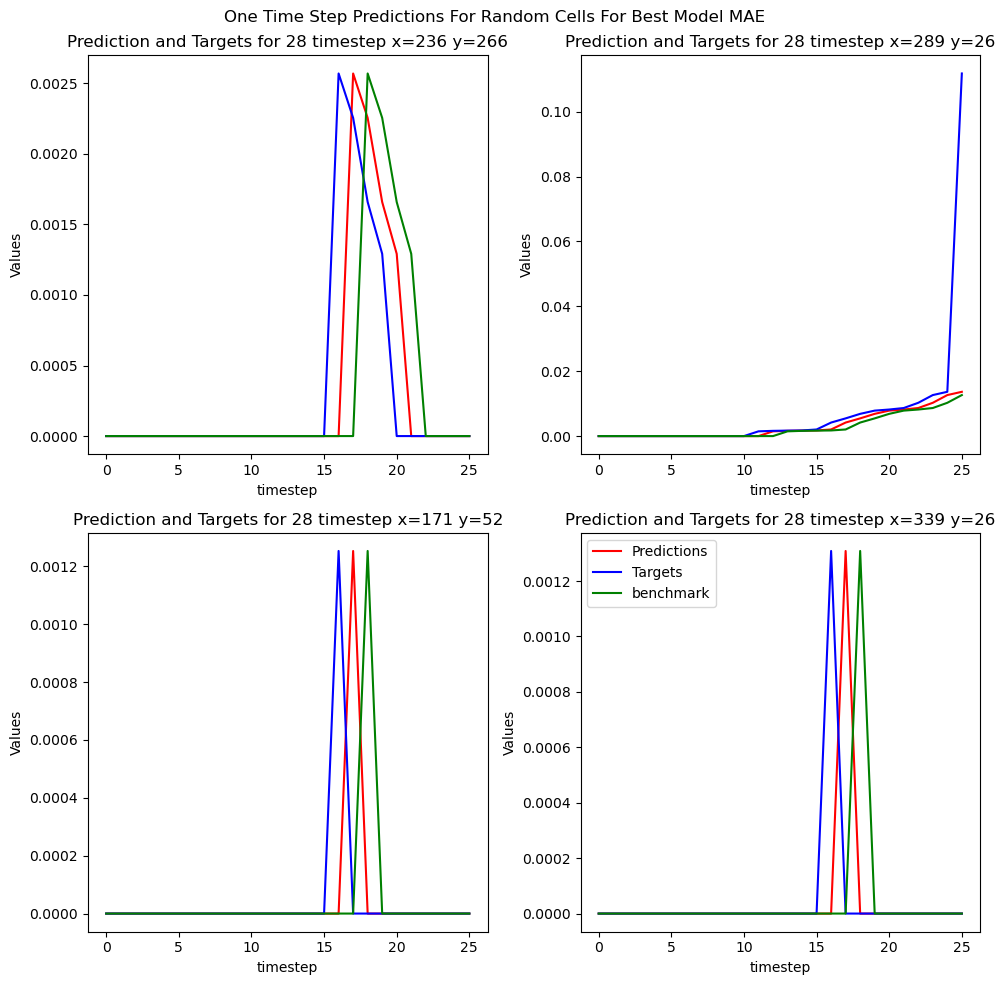
\includegraphics[width=0.8\linewidth, height=0.3\textheight]{Figures/Results/Final_Results/Best_Model_SS_SS_random_cell}
	\caption[Best single time step model on predicting water depth for a single time step]{Best single time step model on predicting water depth for a single time step}
	\label{fig:BSMS}
\end{figure}

Fig. \ref{fig:SpatialTrue} Shows the spatial evolution of water depth on the test set and is used for comparison. Fig. \ref{fig:BMS-spatial} shows the best model from Table \ref{best:ss} and its spatial evolution of water depth over the test set. Fig. \ref{fig:adjusted-spatial} shows the spatial evolution of water depth on the test set using recurrent predictions. All other models predicted 0. This model is a slightly adjusted model, trained on lower epochs (2) and adjusting MAE weighting to 0.5 | 0.5. Fig. \ref{fig:adjusted-recurrent-rc} shows the recurrent preditions of a collection of random cells across the test set.

\begin{figure}[tbph]
	\centering
	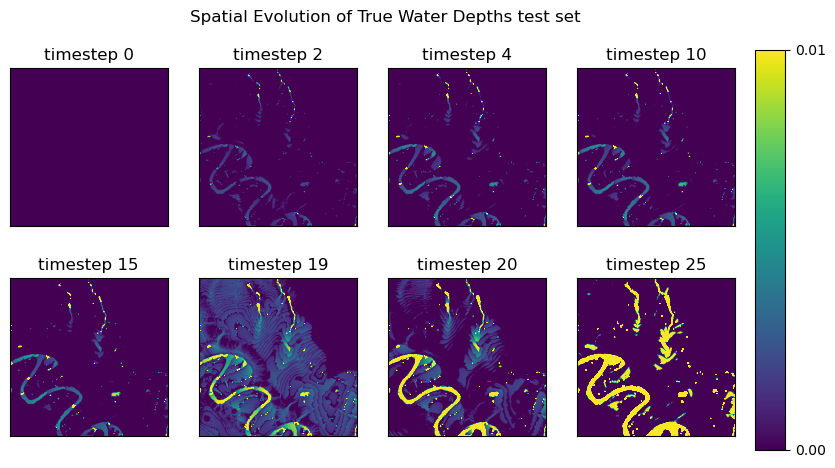
\includegraphics[width=0.8\linewidth, height=0.3\textheight]{Figures/Results/Final_Results/Best_Model_True_test_set}
	\caption[Spatial Evolution of True Water Depth for test set]{Spatial Evolution of True Water Depth for test set}
	\label{fig:SpatialTrue}
\end{figure}


\begin{figure}[tbph]
	\centering
	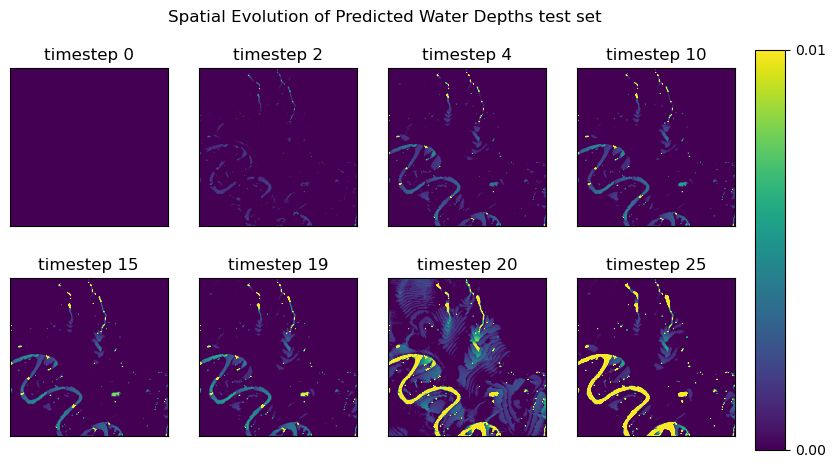
\includegraphics[width=0.8\linewidth, height=0.3\textheight]{Figures/Results/Final_Results/Best_Model_SS_SS_test_set}
	\caption[Spatial Single Time step Predictions]{Spatial Evolution for the Best Model Predicting single time steps}
	\label{fig:BMS-spatial}
\end{figure}


\begin{figure}[tbph]
	\centering
	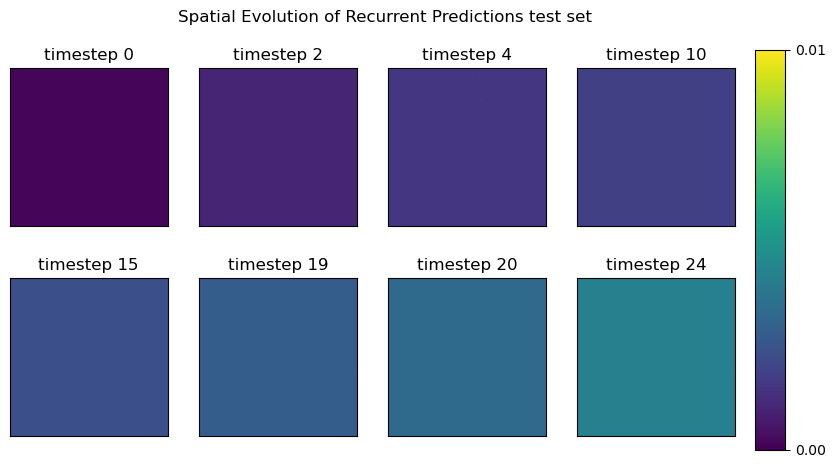
\includegraphics[width=0.8\linewidth, height=0.3\textheight]{Figures/Results/Final_Results/Best_SS_adjusted_weights(5,5)_spatial}
	\caption[Best Model with adjusted weights Spatial recurrent time step Predictions]{Spatial Evolution for the Best Model with adjusted weights (0.5, 0.5) Predicting Recurrent time steps}
	\label{fig:adjusted-spatial}
\end{figure}


\begin{figure}[tbph]
	\centering
	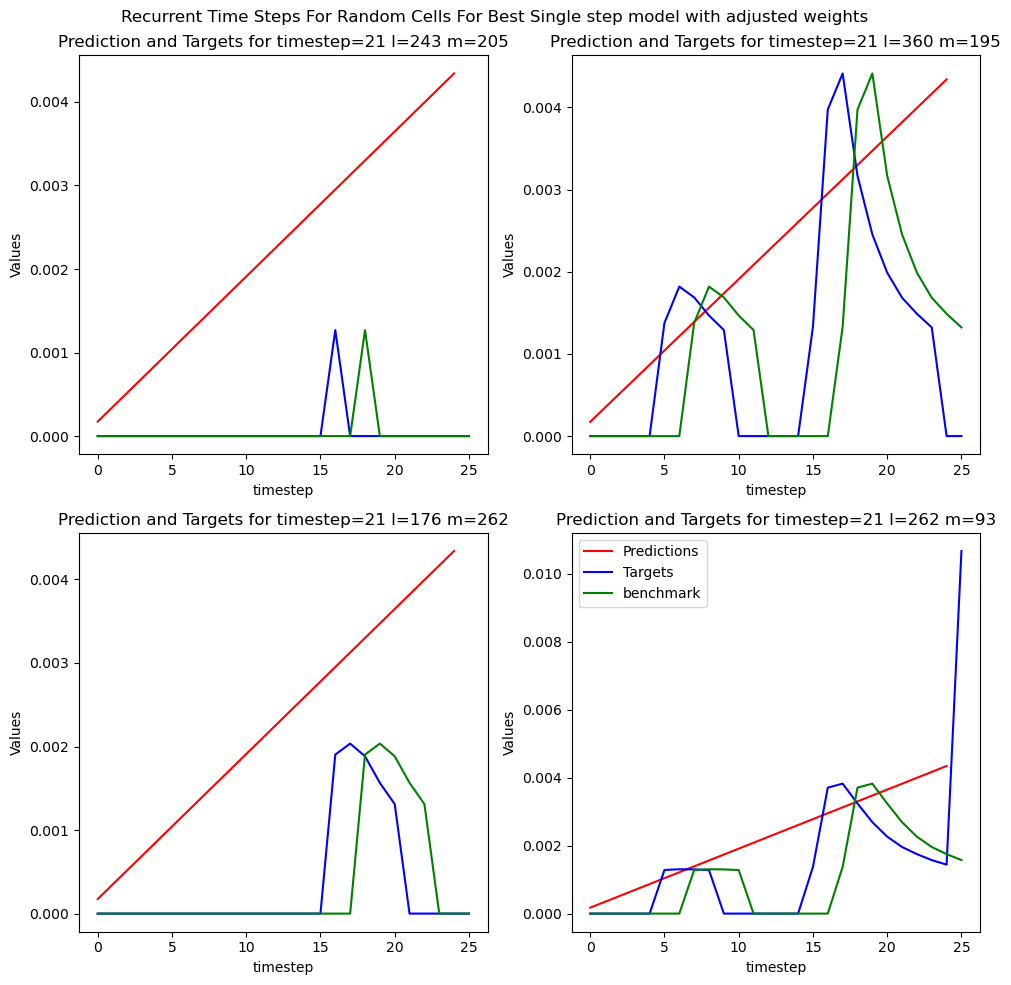
\includegraphics[width=0.8\linewidth, height=0.3\textheight]{Figures/Results/Final_Results/Best_SS_adjusted_weights(5,5)}
	\caption[Spatial Single Time step Predictions]{Spatial Evolution for the Best Model Predicting recurrent time steps but with adjusted weights (0.5, 0.5)}
	\label{fig:adjusted-recurrent-rc}
\end{figure}




